\hypertarget{introduction}{%
\section{Introduction}\label{introduction}}

\begin{quote}
\begin{itemize}
\tightlist
\item[$\square$]
  why inversion attacks on federated learning are important
\item[$\square$]
  why inversion attacks in particular
\item[$\square$]
  why federated learning in particular

  \begin{itemize}
  \tightlist
  \item[$\square$]
    what does federated learning try to solve
  \item[$\square$]
    why should we care about its safety
  \end{itemize}
\end{itemize}

\(\Rightarrow\) We know why we should be concerned with model inversion
on federated learning
\end{quote}

Machine learning models have shown an incredible capacity to interpret
data and deduct from it, enabling numerous breakthroughs by improving
diagnostic capabilities in the medical field {[}@{]}, natural language
processing {[}@{]}, etc. All these applications, however, require
privacy-sensitive data, which has been shown to be inferrable from
trained models (Fredrikson, Jha, and Ristenpart 2015). Federated
Learning attempts to address this and other privacy-related security
issues but is of course not infallible to exploits (Abad et al. 2022).
Federated Learning is relatively new to the space of machine learning
(being introduced in 2015) {[}@{]}, and is already being used in large
enterprises and essential infrastructure. For this reason, cyber attacks
such as Model Inversion could pose a significant, unknown, threat to
users (indirectly) using Federated Learning.

In this essay, I provide an overview of current Model Inversion threats
and defenses to Federated Learning. This overview should serve as an
introduction to Federated Learning and Model Inversion, and assist in
the construction of risk analyses in the context of Federated Learning.
First, I will provide a general overview of Model Inversion methods and
techniques, and introduce Federated Learning and some of the current
threats. This is followed by an overview of different, recent, Model
Inversion attacks on Federated Learning and their respective defenses.
Finally, we will discuss how these developments have influenced the
threat landscape over the last year.

\hypertarget{background}{%
\section{Background}\label{background}}

\begin{quote}
\begin{itemize}
\tightlist
\item[$\square$]
  Introduce Federated Learning from basic principles
\item[$\square$]
  Introduce machine learning exploits, focussing on inference attacks
\item[$\square$]
  Cover the state of FL inference up until last year
\end{itemize}

\(\Rightarrow\) We have a good understanding of FL and inference attacks
\end{quote}

In this section, the necessary background information will be
introduced. The background is considered whatever already existed until
last year (March 2022). We will provide a concise overview of machine
learning principles, to then discuss the workings of Federated Learning
(FL). Having covered the necessary machine learning knowledge, the
discussion will move to how one would attack such systems. Finally, we
focus on previous inference attacks as summarized and discussed by (Abad
et al. 2022).

\hypertarget{machine-learning}{%
\subsection{Machine Learning}\label{machine-learning}}

The goal of any machine learning algorithm is to predict some label or
value given familiar but unseen data. For the purposes of this
discussion, the machine-learning process can be separated into 3 stages:

\begin{enumerate}
\def\labelenumi{\arabic{enumi}.}
\tightlist
\item
  Training
\item
  Testing/Evaluation
\item
  Deployment
\end{enumerate}

During training, the machine learning model, \(f\) is given a set of
tuples \(\{(x_i, y_i)\}\). The learning algorithm then adjusts the model
parameters, \(\theta\), such that it, \(f_\theta\), maps the input
features \(x\) to the target value(s) \(y\). Depending on the learning
task, \(y\) could be a continuous value (regression), a binary value
(binary classification), or a set of discrete values (multi-class
classification) Chakraborty et al. (2018).

The testing phase assesses the performance of the model. We take a
similar, but unseen set of tuples \(\{(x, y)\}\) and test whether the
model, \(f_\theta(x)\) returns the correct value(s). It's important to
only test on \emph{unseen} data since the aim is to assess the
\emph{generalizing} ability of the model. One can imagine the
performance to be higher if the same data that was used to train, was
used to test.

After reaching convergence, when the model does not improve further, it
is deployed to a public, or private, interface.

\hypertarget{federated-learning}{%
\subsection{Federated Learning}\label{federated-learning}}

\begin{quote}
\begin{itemize}
\tightlist
\item[$\square$]
  what is federated learning

  \begin{itemize}
  \tightlist
  \item[$\square$]
    what does it solve
  \item[$\square$]
    how does it work
  \end{itemize}
\end{itemize}

\(\Rightarrow\) We can \textbf{explain how Federated Learning works} and
\textbf{describe the problems it tries to solve}.
\end{quote}

Federated Learning (FL) is a method of delegating, or democratizing, the
training stage of a machine learning algorithm. Its benefits are
threefold (Konečný et al. 2017):

\begin{enumerate}
\def\labelenumi{\arabic{enumi}.}
\tightlist
\item
  It avoids sharing \emph{raw} personal data with a third party.
\item
  Processing resources are delegated.
\item
  Data that is fragmented over multiple locations can still be used for
  training.
\end{enumerate}

The process, generally, works as follows. A set of clients,
\(C={c_0, \ldots, c_n}\), with each their own dataset, train a machine
learning model on that dataset. Information about this trained model is
then sent to a central server that \emph{aggregates} the information
from all clients into a single model. The newly trained model is then
sent back to the clients for another iteration Konečný et al. (2017).

\begin{figure}
\centering
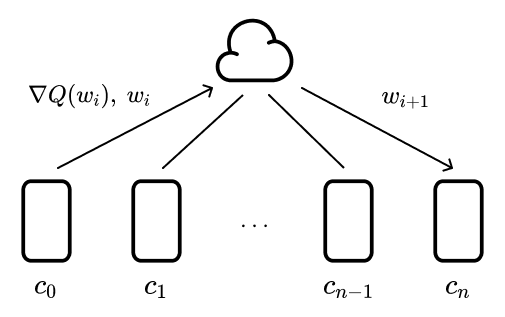
\includegraphics{images/client-server-fl.png}
\caption{Typical Federated Learning network topology. The client,
\(c_i\), sends the gradient, \(\nabla Q(\theta_i)\), and/or weights,
\(\theta_i\), of a particular iteration \(i\). The central server then
sends the updated model parameters \(\theta_{i+1}\) initiating the next
iteration.}
\end{figure}

Various aggregation algorithms exist. The most popular of which are
\emph{Federated Stochastic Gradient Descent} (FedSGD) and
\emph{Federated Averaging} (FedAvg). These both use the \emph{gradient}
(the function that describes how to optimize the model) or the
aforementioned parameters, \(\theta\), of the client models to optimize
the central model Gu, Bai, and Xu (2022). While technical details of
these algorithms are not crucial to this discussion, it is important to
note that this gradient contains information about the distribution of
the client's dataset.

Lastly, there are two types of FL: Horizontal Federated Learning (HFL),
or cross-device Federated Learning; and Vertical Federated Learning
(VFL), or cross-silo Federated Learning Abad et al. (2022). In the
first, devices all collect data on the same features, but their sample
space is not equal (the distributions might not align, and the size can
be different). In the latter, we can imagine a set of hospitals,
companies (or \emph{data silos}) that need to train a model on
\emph{all} the available user data. The data, however, cannot be
directly shared and the data they collect on their users is also
different. Each user is present in each database (they share the same
sample space), but the features on each measurement might be different.
HFL is much more prevalent than VFL {[}@{]}.

\hypertarget{attacking-machine-learning}{%
\subsection{Attacking Machine
Learning}\label{attacking-machine-learning}}

The machine learning approaches discussed so far
(normal/\emph{centralized} learning and Federated Learning) contain
several points at which an attacker could intervene to exploit various
characteristics of the system. Before discussing inference attacks that
take place in later stages of the machine learning pipeline, let us
briefly discuss other potential threats to machine learning models.

The phases discussed in the first section (training, testing, and
deployment) correspond directly to different attacks which can be
categorized as follows (Chakraborty et al. 2018).

\begin{enumerate}
\def\labelenumi{\arabic{enumi}.}
\tightlist
\item
  \emph{Poisoning Attack}: This type of attack, known as contamination
  of the training data, takes place during the training time of the
  machine learning model. An adversary tries to poison the training data
  by injecting carefully designed samples to compromise the whole
  learning process eventually.
\item
  \emph{Evasion Attack}: This is the most common type of attack in the
  adversarial setting. The adversary tries to evade the system by
  adjusting malicious samples during the testing phase. This setting
  does not assume any influence over the training data.
\item
  \emph{Inference/Exploratory Attack}: These attacks do not influence
  any dataset. Given black-box access to the model, they try to gain as
  much knowledge as possible about the learning algorithm of the
  underlying system and pattern in training data.
\end{enumerate}

While the first two also pose potential threats to the FL scheme and are
very popular in centralized machine learning, they are considerably
harder to perform on Federated Learning as the data is distributed
(Tolpegin et al. 2020). Databases of multiple clients have to be
compromised to create an exploit that is comparable to that of a
centralized machine-learning approach.

Inference attacks, however, threaten the privacy guarantees FL attempts
to give. Inference attacks specifically try to \emph{infer} information
about the dataset the model was trained on or the model itself. Thereby
threatening the confidentiality of the database, and thus the privacy,
of the victims involved (Abad et al. 2022). Since they actively infer
information about a deployed system, the amount of information on the
system determines how powerful such an attack could be. For this reason,
they are also further specified as \emph{white-box} or \emph{black-box},
and sometimes \emph{grey-box} inference attacks (Nasr, Shokri, and
Houmansadr 2019).

\hypertarget{inference-attacks}{%
\subsection{Inference Attacks}\label{inference-attacks}}

\begin{quote}
\begin{itemize}
\tightlist
\item[$\square$]
  Give an overview of inference attack classifications
\item[$\square$]
  Provide an example of an inference attack
\end{itemize}

\(\Rightarrow\) We should \textbf{be able to classify different attacks,
understand how they work}, and see \textbf{how they can compromise the
privacy of an individual using the system}
\end{quote}

Inference attacks can be applied to both centralized machine learning
models and Federated Learning schemes. Many of the principles we will
cover apply to both centralized and Federated Learning, but the focus
will be on applications on FL. Specifically, we will provide an overview
of attack classifications as given by (Abad et al. 2022).

Firstly, depending on the target information the attacker attempts to
infer, the attack is classified as follows:

\begin{itemize}
\item
  \emph{Model Inversion}: In model inversion, the attacker attempts to
  invert the machine learning model. Thereby finding the data point
  corresponding to a certain label. (Fredrikson, Jha, and Ristenpart
  2015) were able to invert a facial recognition model, allowing them to
  recover the image of an individual known to be in the training
  dataset.
\item
  \emph{Membership Inference}: In this attack, the goal is to determine
  whether a data point \((x, y)\) was part of the training set. In FL it
  is also possible to determine whether a data point was part of the
  training set of a particular client.
\item
  \emph{Property Inference}: This attack leverages model snapshot
  updates concerning a dataset without the objective property and
  another one containing it. Afterward, a trained binary classifier can
  relate the property with an unseen update, e.g., an update got by
  eavesdropping, to conclude whether the update owns the objective
  property. For a data piece \(x\) containing the property
  \(p: x^{(p)}\) belonging to the dataset \(D_n\) being \(n\) the number
  of clients, the attacker infers if the property belongs to the dataset
  \(x^{(p)} \in D_n\).
\end{itemize}

Secondly, when considering a malicious central server, the attack can be
classified according to the manner in which the attacker interferes with
the training procedure (Abad et al. 2022):

\begin{itemize}
\item
  \emph{Passive}: Also known as an \emph{honest-but-curious} scenario.
  The attacker can only read or eavesdrop on communications (i.e.~the
  weights and gradient transmitted between the clients and the server),
  and the local model and dataset in case of an honest-but-curious
  client.
\item
  \emph{Active}: The attack is more effective than the former but less
  stealthy. It essentially changes the learning goal from minimizing
  loss to maximizing inferred information from the victim.
\end{itemize}

Lastly, attacks can be categorized based on the position of the attacker
in the network:

\begin{itemize}
\item
  \emph{Local}: The attacker is a client, i.e.~they can only access
  \emph{their} database, parameters, and the global parameters they
  receive from the server.
\item
  \emph{Global}: The attacker is the central server. They do not have
  access to any databases but can access the gradients/parameters sent
  by all clients and the global model.
\end{itemize}

\hypertarget{inference-attacks-in-federated-learning}{%
\section{Inference Attacks in Federated
Learning}\label{inference-attacks-in-federated-learning}}

\begin{quote}
\begin{itemize}
\tightlist
\item[$\square$]
  Describe state-of-the-art of model inversion in Federated Learning
\item[$\square$]
  Quickly determine how they relate to other attacks and interpret their
  significance.
\end{itemize}

\(\Rightarrow\) Be able to \textbf{describe the state-of-the-art of
inversion attacks on Federated Learning} and \textbf{describe the risk
profile of each}.
\end{quote}

This section will discuss the state-of-the-art of inference attacks on
Federated Learning. Specifically, we will discuss progress in the field
as of March 2022. The research presented here was found primarily by
querying Google Scholar with the terms ``Inference Attacks on Federated
Learning'', ``Membership Inference on Federated Learning'', ``Model
Inversion on Federated Learning'', and ``Gradient Inversion on Federated
Learning''. The next section will cover the threats these advances pose
to current systems.

First, we will discuss various attacks, focusing not only on their
performance but paying special attention to the scenario in which the
researchers placed the hypothetical adversary. Then, we will cover
defenses to some of these attacks.

\hypertarget{attacking}{%
\subsection{Attacking}\label{attacking}}

Various types of attacks fall under the umbrella of inference attacks.
As of the writing of this essay, the most popular are \emph{Membership
Inference} and \emph{Gradient Inversion} as these show the most results.
\emph{Passive} inference attacks are more often covered than their
\emph{active} counterparts. For each paper, we annotate the type of
attack (see \protect\hyperlink{inference-attacks}{Inference Attacks}),
summarize the findings of the authors, and briefly discuss them.

\hypertarget{do-gradient-inversion-attacks-make-federated-learning-unsafe}{%
\subsubsection{Do Gradient Inversion Attacks Make Federated Learning
Unsafe?}\label{do-gradient-inversion-attacks-make-federated-learning-unsafe}}

Keywords: \emph{Model Inversion}, \emph{Local/Global},
\emph{Cross-Device/HFL}, \emph{Passive}

(Hatamizadeh et al. 2023) performed image reconstruction using gradient
inversion while relaxing a strong assumption made in prior work
regarding Batch Normalization (BN) (Ioffe and Szegedy 2015). BN is a
technique used in neural networks that significantly improve the
learning rate and stability, and is therefore ubiquitous in modern
machine learning. The technique introduces two learned parameters,
\(\beta\) and \(\gamma\), which thus change during the learning
process(Ioffe and Szegedy 2015). Previous work has assumed these
statistics to be static Kaissis et al. (2021), introducing an error that
would compound over time. The authors were able to reliably reconstruct
images without assuming static BN statistics. The authors make a strong
case for an inversion attack that could be used in practice but still
rely on priors (approximations of the image) to make accurate
reconstructions.

\hypertarget{improved-gradient-inversion-attacks-and-defenses-in-federated-learning}{%
\subsubsection{Improved Gradient Inversion Attacks and Defenses in
Federated
Learning}\label{improved-gradient-inversion-attacks-and-defenses-in-federated-learning}}

Keywords: \emph{Membership Inference}, \emph{Local/Global},
\emph{Cross-Device/HFL}, \emph{Passive}, \emph{White-Box}

(Geng et al. 2023) proposed a framework for inverting both
\emph{FedAVG}-based and \emph{FedSGD}-based networks in an
``honest-but-curious'' scenario. They mention prior work has failed to
effectively perform gradient inversion when FL uses the \emph{FedAVG}
aggregation algorithm. Furthermore, they specify methods for fine-tuning
the performance of image restoration in the inverted model, allowing
them to restore images that were introduced 16 epochs before the current
iteration. As Federated Learning is an iterative process, one can
imagine that the further a data point is removed from the current
iteration, the harder it is to infer from the current gradient. While
their results are promising, they do assume a white-box attack scenario
making their attack harder to perform.

\hypertarget{cs-mia-membership-inference-attack-based-on-prediction-confidence-series-in-federated-learning}{%
\subsubsection{CS-MIA: Membership Inference Attack Based on Prediction
Confidence Series in Federated
Learning}\label{cs-mia-membership-inference-attack-based-on-prediction-confidence-series-in-federated-learning}}

Keywords: \emph{Membership Inference}, \emph{Local/Global},
\emph{Cross-Device/VFL}, \emph{Passive}

(Gu, Bai, and Xu 2022) were able to determine whether data points are
members of certain datasets by following the trend in their
classification confidence. Over time, the global model should perform
less well on participant's private data, meaning that member data should
follow a different trend compared to non-member data. They then train a
supervised model the determine whether data points were part of the
training set based on this assumption. The model is then used to
determine the probability of unseen data being part of the target
training data set. They show high accuracy and F1-scores for all
datasets with the lowest performer being MNIST (around 60\% compared to
\textgreater90\% for the other datasets). Still, the proposed solution
scores the best out of all included approaches by a significant margin.

\hypertarget{subject-membership-inference-attacks-in-federated-learning}{%
\subsubsection{Subject Membership Inference Attacks in Federated
Learning}\label{subject-membership-inference-attacks-in-federated-learning}}

Keywords: \emph{Membership Inference}, \emph{Local/Global},
\emph{Cross-Silo/VFL}, \emph{Passive}

In a black-box setting, (Suri et al. 2022) propose a method for what
they call \emph{Subject Inference} (see
\protect\hyperlink{federated-learning}{Federated Learning}). They
describe previous work as being disconnected from real-world scenarios
as it (i) includes information adversaries would not normally have
access to and (ii) assumes the adversary is looking for data points
rather than individuals. Instead of determining whether one particular
data point was part of the training set, the authors attempt to infer
whether an individual, a \_subject, (or rather their distribution) is
present in the dataset given some preexisting information on them. They
show the attack to be very effective in various real-world datasets
while also increasing the realism of the scenario. They show Subject
Inference to be a real threat to user privacy.

\hypertarget{active-membership-inference-attack-under-local-differential-privacy-in-federated-learning.}{%
\subsubsection{Active Membership Inference Attack under Local
Differential Privacy in Federated
Learning.}\label{active-membership-inference-attack-under-local-differential-privacy-in-federated-learning.}}

Keywords: \emph{Membership Inference}, \emph{Local/Global},
\emph{Cross-Device/HFL}, \emph{Active}

Different from other works, (Nguyen et al. 2023) considers a maximally
malicious, i.e.~\emph{active}, membership inference attack. They
implement a method for inferring membership of a particular data point
in the presence of differential privacy (Dwork and Roth 2013).
Differential privacy obscures the relation of the individual to the data
point, without affecting the patterns used for training machine learning
models. The authors show that their method performs well, even under
such obscuring of the data. Furthermore, the attack only starts to
degrade after the level of obscurity interferes with model performance.
They show that more rigorous privacy methods should be proposed to deal
with such attacks.

\hypertarget{defending}{%
\subsection{Defending}\label{defending}}

\begin{quote}
\begin{itemize}
\tightlist
\item[$\square$]
  How can some of the aforementioned attacks be prevented or their risks
  reduced
\item[$\square$]
  What are the trade-offs, and do they make any implicit/explicit
  assumptions?
\end{itemize}

\(\Rightarrow\) We can \textbf{describe some tactics to mitigate the
impact of the aforementioned attacks} and \textbf{use them in the
context of a cost/benefit analysis}
\end{quote}

To combat inference attacks, we discuss potential defenses against them.
Some of the papers that are included have been discussed in the last
section. These have been marked with a footnote accordingly \footnote{Often,
  novel attack proposals also include possible countermeasures. Some of
  the papers covered in the last section, therefore, have also been
  included in this section.}. For each paper, we will summarize the
proposed measures and briefly discuss them.

\hypertarget{improved-gradient-inversion-attacks-and-defenses-in-federated-learning1}{%
\subsubsection[Improved Gradient Inversion Attacks and Defenses in
Federated Learning]{\texorpdfstring{Improved Gradient Inversion Attacks
and Defenses in Federated
Learning\footnote{Often, novel attack proposals also include possible
  countermeasures. Some of the papers covered in the last section,
  therefore, have also been included in this section.}}{Improved Gradient Inversion Attacks and Defenses in Federated Learning}}\label{improved-gradient-inversion-attacks-and-defenses-in-federated-learning1}}

(Geng et al. 2023) found that labels that only appeared only once were
more prone to their proposed inversion attacks (see
\protect\hyperlink{improved-gradient-inversion-attacks-and-defenses-in-federated-learning}{}).
They also mention the use of larger batch sizes in the global model
(i.e.~more clients) to reduce the amount of private information embedded
in a single batch. Lastly, they claim FedAVG possesses ``stronger
privacy preserving capabilities than FedSGD''. As this was included in
the discussion of their attack-oriented paper, they do not evaluate
these claims further.

\hypertarget{do-gradient-inversion-attacks-make-federated-learning-unsafe1}{%
\subsubsection[Do Gradient Inversion Attacks Make Federated Learning
Unsafe?]{\texorpdfstring{Do Gradient Inversion Attacks Make Federated
Learning
Unsafe?\footnote{Often, novel attack proposals also include possible
  countermeasures. Some of the papers covered in the last section,
  therefore, have also been included in this section.}}{Do Gradient Inversion Attacks Make Federated Learning Unsafe?}}\label{do-gradient-inversion-attacks-make-federated-learning-unsafe1}}

(Hatamizadeh et al. 2023) make several recommendations to make existing
implementations of FL safer, namely: (i) larger training sets, (ii)
updates from a larger number of iterations over different (iii) large
batch sizes. In addition, they mention three more changes that could
potentially mitigate server-side (i.e.~\emph{Global}) gradient inversion
attacks: (1) The use of \emph{Homomorphic Encryption} (see
\protect\hyperlink{discussion}{Discussion}), (2) ensuring the attacker
does not have knowledge of the model architecture, and (3) using an
alternative aggregation algorithm such as FedBN Andreux et al. (2020).
The countermeasures provided are relatively general. They also provided
sources affirming their suspicions.

\hypertarget{an-empirical-analysis-of-image-augmentation-against-model-inversion-attack-in-federated-learning}{%
\subsubsection{An Empirical Analysis of Image Augmentation Against Model
Inversion Attack in Federated
Learning}\label{an-empirical-analysis-of-image-augmentation-against-model-inversion-attack-in-federated-learning}}

(Shin et al. 2023) propose the use of image augmentation as a more
viable alternative to differential privacy (Dwork and Roth 2013). Image
augmentation is a data synthesis method that increases the size of the
training set, and reduces over-fitting (Shorten and Khoshgoftaar 2019).
As this introduces fake data while improving the over-all performance of
the model, the authors suggest it could be used to mitigate model
inversion attacks. They attack they used was introduced by (Geiping et
al. 2020), and various more successful attacks have been constructed
since then Geng et al. (2023).

\hypertarget{ressfl-a-resistance-transfer-framework-for-defending-model-inversion-attack-in-split-federated-learning}{%
\subsubsection{ResSFL: A Resistance Transfer Framework for Defending
Model Inversion Attack in Split Federated
Learning}\label{ressfl-a-resistance-transfer-framework-for-defending-model-inversion-attack-in-split-federated-learning}}

In a framework introduced by (J. Li et al. 2022), Split Federated
Learning (SFL) (Annavaram and Avestimehr, n.d.) is augmented with an
discriminator-like model that attempts to invert the model before the
client sends their model to the central server. By choosing weights
where the discriminator performs poorly, they claim to improve the
resiliency of the scheme to model inversion attacks. They indeed show
improvements over the standard implementation of SFL, but do not mention
how this method compares to attacks on default FL.

\hypertarget{discussion}{%
\section{Discussion}\label{discussion}}

\begin{quote}
\begin{itemize}
\tightlist
\item[$\square$]
  What can we say about the threat these attacks pose?

  \begin{itemize}
  \tightlist
  \item[$\square$]
    How effective are these defenses?
  \item[$\square$]
    What is the trade-off?
  \end{itemize}
\item[$\square$]
  What research can be done to mitigate these risks?
\end{itemize}

\(\Rightarrow\) We \textbf{understand what the current threat landscape
for IA on FL looks like} and \textbf{know where to improve understanding
to mitigate the risks}.
\end{quote}

In this section, we will discuss the attacks and defenses as presented
in the last section. Specifically, we determine the threats these
attacks pose and if the defenses included could effectively mitigate
the. In the end, we propose new research directions that could help
mitigate these threats.

\hypertarget{current-threats-and-trends}{%
\subsection{Current Threats and
Trends}\label{current-threats-and-trends}}

The attacks presented show how Federated Learning might not be able to
guarantee privacy. Privacy, thus, should still remain a concern even if
Federated Learning brings stronger privacy guarantees than traditional
machine learning and its derivatives. Let us summarize the threats these
attacks pose:

\begin{itemize}
\item
  \emph{More Realistic Scenarios}: Research starts to introduce more
  realistic scenarios that could threaten current implementations of
  Federated Learning. As the field matures, attacks seem to become more
  realistic. Especially the work presented by (Suri et al. 2022) poses a
  real threat as it assumes a complete black-box attack with reasonable
  assumptions while still showing good performance. Even in complete
  black-box settings, however, we still assume the ability to intercept
  and read the communications. Were this to be encrypted, such attacks
  could possibly be mitigated (Y. Li et al. 2021).
\item
  \emph{Increased Resilience Against Existing Privacy Measures}: Some of
  the aforementioned papers have shown improvements concerning the
  evasion of privacy-preserving measures.
\end{itemize}

\hypertarget{future-work}{%
\subsection{Future Work}\label{future-work}}

\hypertarget{conclusion}{%
\section{Conclusion}\label{conclusion}}

\begin{quote}
\begin{itemize}
\tightlist
\item[$\square$]
  How `risky' are the tactics described in this essay
\item[$\square$]
  Do the defenses have any real impact on the risk of these attacks
\item[$\square$]
  What would we need to research to improve any of these risks
\end{itemize}

\(\Rightarrow\) We can \textbf{describe the overall risk of model
inversion attacks on federated learning} and \textbf{build on top of
this paper to reduce their risks and improve our understanding}
\end{quote}

\hypertarget{references}{%
\section*{References}\label{references}}
\addcontentsline{toc}{section}{References}

\hypertarget{refs}{}
\begin{CSLReferences}{1}{0}
\leavevmode\vadjust pre{\hypertarget{ref-abadSecurityPrivacyFederated2022}{}}%
Abad, Gorka, Stjepan Picek, Víctor Julio Ramírez-Durán, and Aitor
Urbieta. 2022. {``On the {Security} \& {Privacy} in {Federated
Learning}.''} {arXiv}. \url{https://arxiv.org/abs/2112.05423}.

\leavevmode\vadjust pre{\hypertarget{ref-andreuxSiloedFederatedLearning2020}{}}%
Andreux, Mathieu, Jean Ogier Du Terrail, Constance Beguier, and Eric W.
Tramel. 2020. {``Siloed {Federated Learning} for {Multi-centric
Histopathology Datasets}.''} In \emph{Domain {Adaptation} and
{Representation Transfer}, and {Distributed} and {Collaborative
Learning}}, edited by Shadi Albarqouni, Spyridon Bakas, Konstantinos
Kamnitsas, M. Jorge Cardoso, Bennett Landman, Wenqi Li, Fausto
Milletari, et al., 12444:129--39. {Cham}: {Springer International
Publishing}. \url{https://doi.org/10.1007/978-3-030-60548-3_13}.

\leavevmode\vadjust pre{\hypertarget{ref-annavaramGroupKnowledgeTransfer}{}}%
Annavaram, Chaoyang He Murali, and Salman Avestimehr. n.d. {``Group
{Knowledge Transfer}: {Federated Learning} of {Large CNNs} at the
{Edge}.''}

\leavevmode\vadjust pre{\hypertarget{ref-chakrabortyAdversarialAttacksDefences2018}{}}%
Chakraborty, Anirban, Manaar Alam, Vishal Dey, Anupam Chattopadhyay, and
Debdeep Mukhopadhyay. 2018. {``Adversarial {Attacks} and {Defences}: {A
Survey}.''} {arXiv}. \url{https://arxiv.org/abs/1810.00069}.

\leavevmode\vadjust pre{\hypertarget{ref-dworkAlgorithmicFoundationsDifferential2013}{}}%
Dwork, Cynthia, and Aaron Roth. 2013. {``The {Algorithmic Foundations}
of {Differential Privacy}.''} \emph{Foundations and
Trends\textregistered{} in Theoretical Computer Science} 9 (3-4):
211--407. \url{https://doi.org/10.1561/0400000042}.

\leavevmode\vadjust pre{\hypertarget{ref-fredriksonModelInversionAttacks2015}{}}%
Fredrikson, Matt, Somesh Jha, and Thomas Ristenpart. 2015. {``Model
{Inversion Attacks} That {Exploit Confidence Information} and {Basic
Countermeasures}.''} In \emph{Proceedings of the 22nd {ACM SIGSAC
Conference} on {Computer} and {Communications Security}}, 1322--33.
{CCS} '15. {New York, NY, USA}: {Association for Computing Machinery}.
\url{https://doi.org/10.1145/2810103.2813677}.

\leavevmode\vadjust pre{\hypertarget{ref-geipingInvertingGradientsHow2020}{}}%
Geiping, Jonas, Hartmut Bauermeister, Hannah Dröge, and Michael Moeller.
2020. {``Inverting {Gradients} - {How} Easy Is It to Break Privacy in
Federated Learning?''} In \emph{Advances in {Neural Information
Processing Systems}}, 33:16937--47. {Curran Associates, Inc.}

\leavevmode\vadjust pre{\hypertarget{ref-gengImprovedGradientInversion2023}{}}%
Geng, Jiahui, Yongli Mou, Qing Li, Feifei Li, Oya Beyan, Stefan Decker,
and Chunming Rong. 2023. {``Improved {Gradient Inversion Attacks} and
{Defenses} in {Federated Learning}.''} \emph{IEEE Transactions on Big
Data}, 1--13. \url{https://doi.org/10.1109/TBDATA.2023.3239116}.

\leavevmode\vadjust pre{\hypertarget{ref-guCSMIAMembershipInference2022}{}}%
Gu, Yuhao, Yuebin Bai, and Shubin Xu. 2022. {``{CS-MIA}: {Membership}
Inference Attack Based on Prediction Confidence Series in Federated
Learning.''} \emph{Journal of Information Security and Applications} 67
(June): 103201. \url{https://doi.org/10.1016/j.jisa.2022.103201}.

\leavevmode\vadjust pre{\hypertarget{ref-hatamizadehGradientInversionAttacks2023}{}}%
Hatamizadeh, Ali, Hongxu Yin, Pavlo Molchanov, Andriy Myronenko, Wenqi
Li, Prerna Dogra, Andrew Feng, et al. 2023. {``Do {Gradient Inversion
Attacks Make Federated Learning Unsafe}?''} \emph{IEEE Transactions on
Medical Imaging}, 1--1. \url{https://doi.org/10.1109/TMI.2023.3239391}.

\leavevmode\vadjust pre{\hypertarget{ref-ioffeBatchNormalizationAccelerating2015}{}}%
Ioffe, Sergey, and Christian Szegedy. 2015. {``Batch {Normalization}:
{Accelerating Deep Network Training} by {Reducing Internal Covariate
Shift}.''} {arXiv}. \url{https://doi.org/10.48550/arXiv.1502.03167}.

\leavevmode\vadjust pre{\hypertarget{ref-kaissisEndtoendPrivacyPreserving2021}{}}%
Kaissis, Georgios, Alexander Ziller, Jonathan Passerat-Palmbach, Théo
Ryffel, Dmitrii Usynin, Andrew Trask, Ionésio Lima, et al. 2021.
{``End-to-End Privacy Preserving Deep Learning on Multi-Institutional
Medical Imaging.''} \emph{Nature Machine Intelligence} 3 (6): 473--84.
\url{https://doi.org/10.1038/s42256-021-00337-8}.

\leavevmode\vadjust pre{\hypertarget{ref-konecnyFederatedLearningStrategies2017}{}}%
Konečný, Jakub, H. Brendan McMahan, Felix X. Yu, Peter Richtárik, Ananda
Theertha Suresh, and Dave Bacon. 2017. {``Federated {Learning}:
{Strategies} for {Improving Communication Efficiency}.''} {arXiv}.
\url{https://doi.org/10.48550/arXiv.1610.05492}.

\leavevmode\vadjust pre{\hypertarget{ref-liResSFLResistanceTransfer2022}{}}%
Li, Jingtao, Adnan Siraj Rakin, Xing Chen, Zhezhi He, Deliang Fan, and
Chaitali Chakrabarti. 2022. {``{ResSFL}: {A Resistance Transfer
Framework} for {Defending Model Inversion Attack} in {Split Federated
Learning}.''} In \emph{Proceedings of the {IEEE}/{CVF Conference} on
{Computer Vision} and {Pattern Recognition}}, 10194--202.

\leavevmode\vadjust pre{\hypertarget{ref-liFedBNFederatedLearning2021}{}}%
Li, Xiaoxiao, Meirui Jiang, Xiaofei Zhang, Michael Kamp, and Qi Dou.
2021. {``{FedBN}: {Federated Learning} on {Non-IID Features} via {Local
Batch Normalization}.''} {arXiv}.
\url{https://doi.org/10.48550/arXiv.2102.07623}.

\leavevmode\vadjust pre{\hypertarget{ref-liPrivacyThreatsAnalysis2021}{}}%
Li, Yuchen, Yifan Bao, Liyao Xiang, Junhan Liu, Cen Chen, Li Wang, and
Xinbing Wang. 2021. {``Privacy {Threats Analysis} to {Secure Federated
Learning}.''} {arXiv}. \url{https://arxiv.org/abs/2106.13076}.

\leavevmode\vadjust pre{\hypertarget{ref-nasrComprehensivePrivacyAnalysis2019}{}}%
Nasr, Milad, Reza Shokri, and Amir Houmansadr. 2019. {``Comprehensive
{Privacy Analysis} of {Deep Learning}: {Passive} and {Active White-box
Inference Attacks} Against {Centralized} and {Federated Learning}.''} In
\emph{2019 {IEEE Symposium} on {Security} and {Privacy} ({SP})},
739--53. \url{https://doi.org/10.1109/SP.2019.00065}.

\leavevmode\vadjust pre{\hypertarget{ref-nguyenActiveMembershipInference2023}{}}%
Nguyen, Truc, Phung Lai, Khang Tran, NhatHai Phan, and My T. Thai. 2023.
{``Active {Membership Inference Attack} Under {Local Differential
Privacy} in {Federated Learning}.''} {arXiv}.
\url{https://doi.org/10.48550/arXiv.2302.12685}.

\leavevmode\vadjust pre{\hypertarget{ref-shinEmpiricalAnalysisImage2023}{}}%
Shin, Seunghyeon, Mallika Boyapati, Kun Suo, Kyungtae Kang, and Junggab
Son. 2023. {``An Empirical Analysis of Image Augmentation Against Model
Inversion Attack in Federated Learning.''} \emph{Cluster Computing} 26
(1): 349--66. \url{https://doi.org/10.1007/s10586-022-03596-1}.

\leavevmode\vadjust pre{\hypertarget{ref-shortenSurveyImageData2019}{}}%
Shorten, Connor, and Taghi M. Khoshgoftaar. 2019. {``A Survey on {Image
Data Augmentation} for {Deep Learning}.''} \emph{Journal of Big Data} 6
(1): 60. \url{https://doi.org/10.1186/s40537-019-0197-0}.

\leavevmode\vadjust pre{\hypertarget{ref-suriSubjectMembershipInference2022}{}}%
Suri, Anshuman, Pallika Kanani, Virendra J. Marathe, and Daniel W.
Peterson. 2022. {``Subject {Membership Inference Attacks} in {Federated
Learning}.''} \emph{arXiv.org}. https://arxiv.org/abs/2206.03317v3.

\leavevmode\vadjust pre{\hypertarget{ref-tolpeginDataPoisoningAttacks2020}{}}%
Tolpegin, Vale, Stacey Truex, Mehmet Emre Gursoy, and Ling Liu. 2020.
{``Data {Poisoning Attacks Against Federated Learning Systems}.''}
\emph{arXiv.org}. https://arxiv.org/abs/2007.08432v2.

\end{CSLReferences}
